\documentclass[aspectratio=169, 8pt,t]{beamer}
\graphicspath{{figures/}} % Setting the graphicspath

% Theme settings
\usetheme{Madrid}
\usecolortheme{default}
\setbeamertemplate{navigation symbols}{}   % removes navigation symbols such as 'next page'
\setbeamertemplate{footline}{}             % remove line with name, date, page nr.
\setbeamercolor*{frametitle}{bg=white}     % remove background from frametitle
\usepackage{caption}
% \captionsetup[figure]{labelformat=empty}% redefines the caption setup of the figures environment in the beamer class.
\setbeamersize{text margin left=20pt,text margin right=10pt}
\usefonttheme[onlymath]{serif} % makes beamer math look like article math
\usepackage{hyperref}

%======================= title page info =======================
\title{An NNPDF4.0 determination of $\alpha_s$ -- methodologies \& status}
\date{NNPDF collaboration meeting  \\[0.1cm] Amsterdam, 24 February 2024}
\author{Roy Stegeman}
\institute{\small The University of Edinburgh}


%======================= page numbering =======================
\addtobeamertemplate{navigation symbols}{}{ \usebeamerfont{footline}
  \insertframenumber / \inserttotalframenumber \hspace*{2mm} \\ \vspace*{1mm}
}


%=================================== colors ====================================
\definecolor{RoyBlue}{RGB}{22, 46, 69}
\definecolor{RoyGrey}{RGB}{64, 88, 128}

\newcommand{\hlme}[1]{{\color{red}\bf #1}} % highlight me

\setbeamercolor{structure}{fg=RoyBlue} % itemize, enumerate, etc
\setbeamercolor{frametitle}{fg=RoyGrey}
\setbeamercolor{section in head/foot}{bg=RoyBlue}


%======================= add progress dots to headline =========================
\setbeamertemplate{headline}{%
    \begin{beamercolorbox}[ht=4mm,dp=4mm]{section in head/foot}
        \insertnavigation{\paperwidth}
    \end{beamercolorbox}%
}%
\makeatother


%======================= add section title page ================================
\AtBeginSection[]{
  \begin{frame}
  \vfill
  \centering
    \usebeamerfont{title}\insertsection\par%
  \vfill
  \end{frame}
}


%=================================== titlepage =================================
\titlegraphic{\vspace*{6mm}
  
\includegraphics[height=1.5cm]{logos/edi_logo.png} \hspace{10mm}
  % 
\includegraphics[height=0.8cm]{logos/nnpdf_logo_official.pdf} \hspace{10mm}
  
\includegraphics[height=1.5cm]{logos/higgs_logo.jpg}
}

\defbeamertemplate{title page}{noinstitute}[1][]
{
  \vbox{}
  \vfill
  \begingroup
    \centering
    \begin{beamercolorbox}[sep=8pt,center,#1]{title}
      \usebeamerfont{title}\inserttitle\par%
      \ifx\insertsubtitle\@empty%
      \else%
        \vskip0.25em%
        {\usebeamerfont{subtitle}\usebeamercolor[fg]{subtitle}\insertsubtitle\par}%
      \fi%
    \end{beamercolorbox}%
    \vskip2em\par
    \begin{beamercolorbox}[sep=0pt,center,#1]{author}
      \usebeamerfont{author}\insertauthor
    \end{beamercolorbox}
  \begin{beamercolorbox}[sep=0pt,center,#1]{author}
    \usebeamerfont{institute}\insertinstitute
  \end{beamercolorbox}
  \vspace*{8pt}
  \vspace*{16pt}
    \begin{beamercolorbox}[sep=0pt,center,#1]{date}
      \usebeamerfont{date}\insertdate
    \end{beamercolorbox}\vskip0.5em
    {\usebeamercolor[fg]{titlegraphic}\inserttitlegraphic\par}
  \endgroup
  \vfill
}

\makeatletter
\setbeamertemplate{title page}[noinstitute][colsep=-4bp,rounded=true,shadow=\beamer@themerounded@shadow]
\makeatother


\begin{document}
{
\setbeamertemplate{headline}{} % remove headline from titlepage
\begin{frame}
  \titlepage
\end{frame}
}

\setbeamertemplate{enumerate items}[default]

\pgfdeclarelayer{bg}    % declare background layer
\pgfsetlayers{bg,main}  % set the order of the layers (main is the standard layer)


% SLIDES =======================================================================

\begin{frame}{Status of $\alpha_s$ determinations (as of August 2021, largely the same today)}
    \vspace*{-1em}
    \begin{figure}
      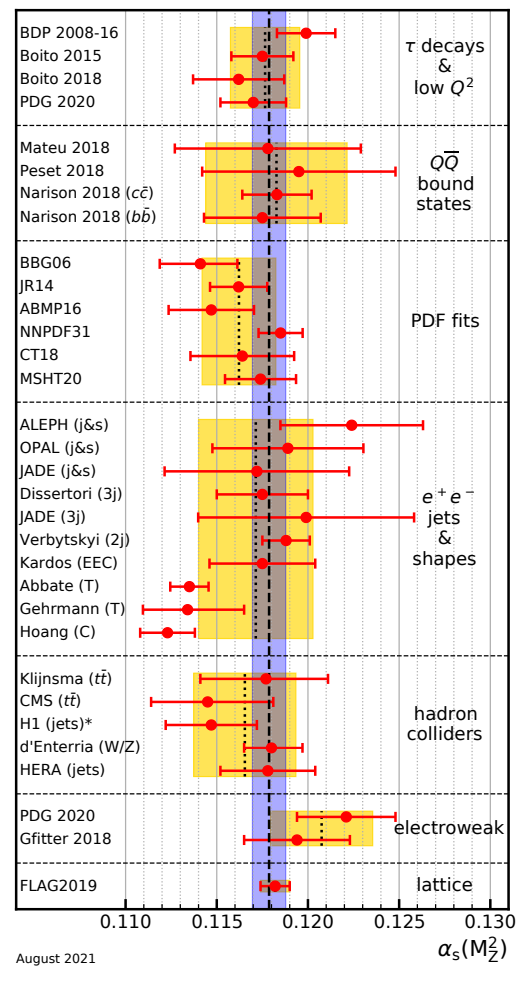
\includegraphics[width=0.25\textwidth]{pdg_alphas.png}
    \end{figure}
\end{frame}

\begin{frame}{Status of $\alpha_s$ determinations (as of August 2021, largely the same today)}
  \vspace*{-1em}
  \begin{figure}
    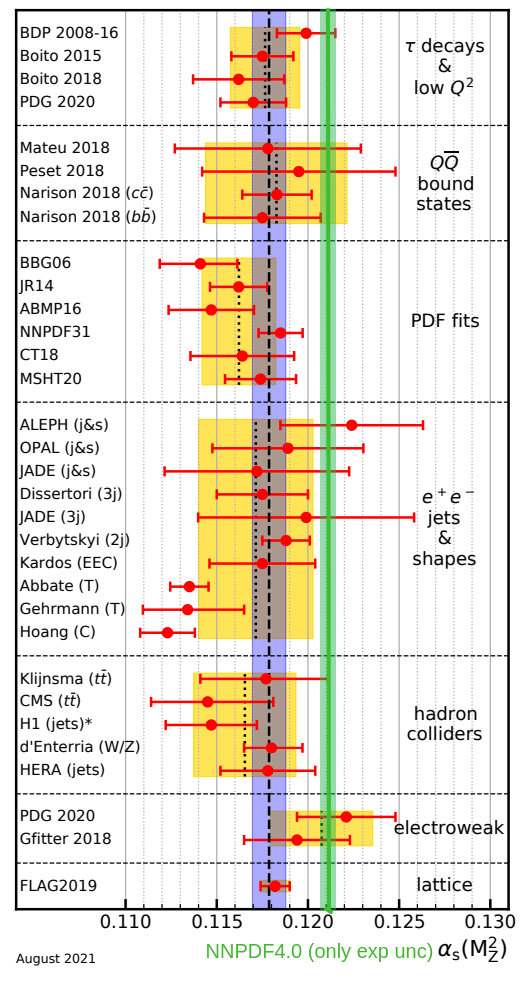
\includegraphics[width=0.25\textwidth]{pdf_alphas_updated.png}
  \end{figure}
\end{frame}


\begin{frame}{Three different methodologies}
  \begin{itemize}
    \item Correlated replica method \href{https://arxiv.org/abs/1802.03398}{\textcolor{gray}{[NNPDF Collaboration (2018); 1802.03398]}}
    \item Theory covariance method \href{https://arxiv.org/abs/2105.05114}{\textcolor{gray}{[Ball \& Pearson (2021); 2105.05114]}}
    \item SIMUnet (no results in these slides) \href{https://arxiv.org/abs/2201.07240}{\textcolor{gray}{[Iranipour \& Ubiali (2022); 2201.07240]}}
  \end{itemize}
\end{frame}


\begin{frame}{Correlated replica method}{Methodology}
  Determining $\alpha_s$ with a fixed input PDF results in underestimated uncertainty
  \begin{figure}
    \centering
    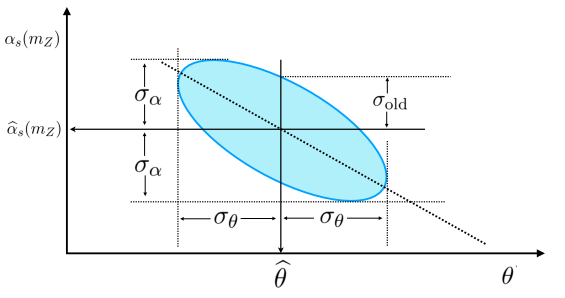
\includegraphics[width=0.7\textwidth]{figures/alphaspdfcorplot.png}
  \end{figure}
\end{frame}


\begin{frame}{Correlated replica method}{Methodology}
  \begin{columns}
    \column{0.5\textwidth}
    1. Produce fits to a data replica, $D^{(k)}$, at different values of $\alpha_s$\\\vspace*{1em}
    2. Perform quadratic fits to $\chi^{2(k)}(\alpha_s)$ profiles \\
    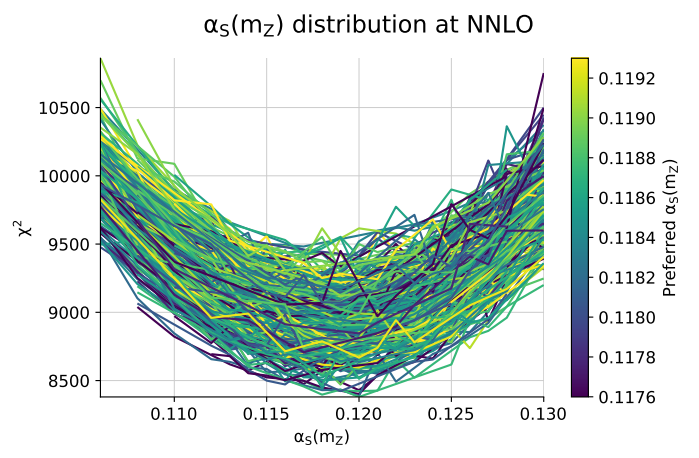
\includegraphics[width=0.9\textwidth]{figures/parabolaplotnnpdf31.png}
    \column{0.5\textwidth}
    3. Compute $\alpha_s^{(k)}=\operatorname{argmin}\left[\chi^{2(k)}\left(\alpha_s\right)\right]$  for each replica $k$ \\
    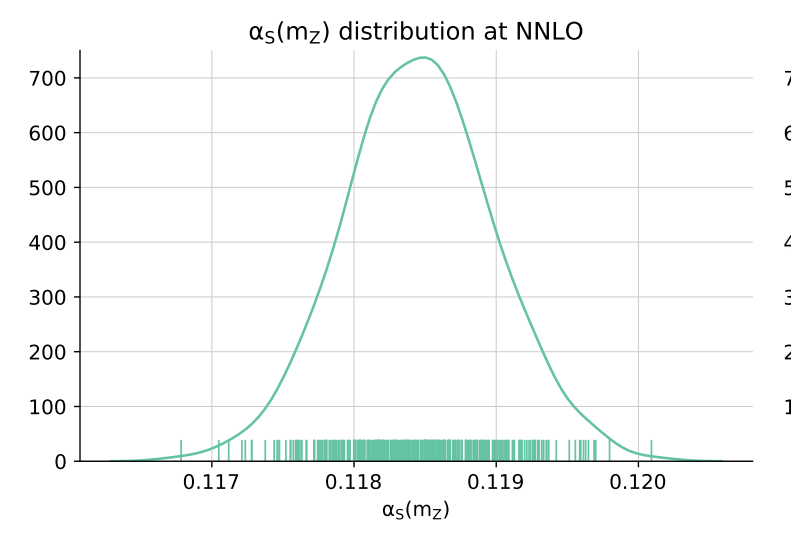
\includegraphics[width=0.9\textwidth]{figures/alphasnnpdf31result.png}
  \end{columns}
\end{frame}


\begin{frame}{Correlated replica method}{Sources of uncertainty}
  \begin{itemize}
    \item Experimental uncertainties
    \item Theory uncertainties
    \begin{itemize}
      \item Choice regarding construction of MHOU covmat, e.g. which value of $\alpha_s$, impact of scale variation magnitude
    \end{itemize}
    \item Methodological uncertainty:
    \begin{itemize}
      \item Selection of replicas (postfit may remove some points in $\alpha_s$)
      \item Finite size uncertainty due to finite number of replicas
      \item Grid of fitted $\alpha_s$ values
      \item Number of batches
      \item Choice of parabolic $\chi^2(\alpha_s)$ profile
      \item Dependence on $t0$-PDF
      \item \ldots did I forget any?
    \end{itemize}
  \end{itemize}
\end{frame}


\begin{frame}{Correlated replica method}{Results}
  NNPDF3.1: 0.1183 ± 0.0007 (a single batch)

  \vspace*{1em}
  NNPDF4.0 methodology and dataset (new pipeline):
  \begin{enumerate}
    \item Compute NNLO Fktables at $\alpha_s\in \{0.114,0.115,0.116,0.117,0.118,0.119,0.120,0.121,0.122\}$
    \item Generate 200 replica PDF at each $\alpha_s$
    \item Iterate preprocessing, but for all iterated $\alpha_s$ fits take $t0$-PDF from the $\alpha_s=0.118$ fit of the previous iteration
    \item[3a.] In case of MHOU, include the MHOU covmat computed at $\alpha_s=0.118$
    \item fit $\chi^2$ profile using a second order polynomial only to the data replicas for which all $\alpha_s$ values passed postfit selection
    \item Collect statistics of minima of the parabola
  \end{enumerate}
\end{frame}


\begin{frame}{Correlated replica method}{Results}
  NNPDF3.1: 0.1183 ± 0.0007 (a single batch)

  \vspace*{1em}
  NNPDF4.0 methodology and dataset (new pipeline):
  \begin{figure}
    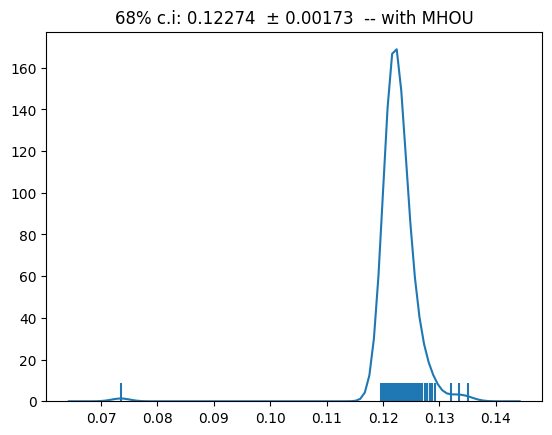
\includegraphics[width=0.25\textwidth]{withmhou_kdeplot.png}
    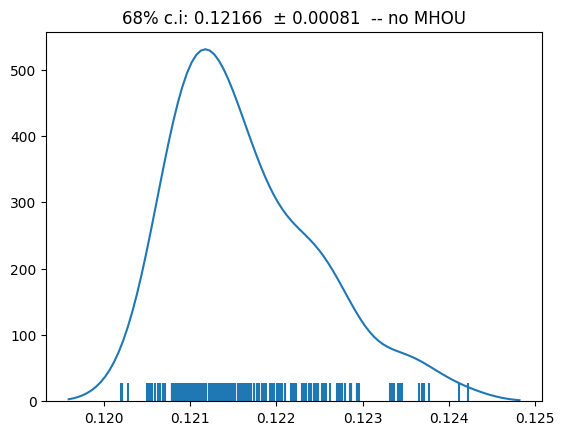
\includegraphics[width=0.25\textwidth]{nomhou_kdeplot.png}
  \end{figure}
  Including MHOU increases uncertainty on $\alpha_s$ by an amount that is similar to the estimated theory uncertainty in the NNPDF3.1 $\alpha_s$ determination where it was 0.0011

  \vspace*{0.5em}
  The MHOU determination displays large non-Gaussianity that we will need to control

  \vspace*{0.5em}
  The central value is still high, even outside the grid of FKtables for MHOU
\end{frame}


\begin{frame}{Correlated replica method}{Results}
  Let us use the ``old'' methodology of NNPDF2.1 \href{https://arxiv.org/abs/1110.2483}{\textcolor{gray}{[NNPDF Collaboration (2011); 1110.2483]}}

  \begin{figure}
    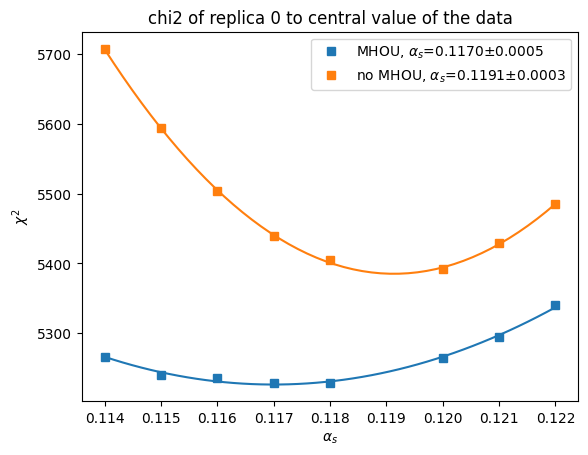
\includegraphics[width=0.35\textwidth]{naivechi2fit.png}
  \end{figure}
  \centering
  Compared to 0.12274$\pm$0.00173 (MHOU) and 0.12166$\pm$0.00081 (no MHOU)

  \vspace*{0.5em}
  Why do the old and new correlated replica methods disagree?
\end{frame}


\begin{frame}{Theory covariance method}{Results}
  Same method as introduced by Amedeo, but now applied to $\alpha_s$

  \vspace*{0.5em}
  3pt scale variations: [0.114; 0.118; 0.122]

  \vspace*{2em}

  \begin{table}[]
    \begin{tabular}{llll}
    \textbf{Data set} & \textbf{Methodological details} & \textbf{Corr. reps. meth.} & \textbf{Theory cov. meth.}       \\
    NNPDF4.0          & NNPDF4.0                        & 0.12166 ± 0.00081          & {0.11965 ± 0.00036} \\
    NNPDF4.0          & NNPDF4.0 + MHOU                 & 0.12274 ± 0.00173          & {0.11914 ± 0.00070}
    \end{tabular}
  \end{table}

  \vspace*{1em}
  Small uncertainty, even with MHOU included

  \vspace*{0.5em}
  Disagreement between both methodologies

\end{frame}



\begin{frame}{Way forward?}
  Challenges:
  \begin{itemize}
    \item Disagreement between datasets (still to confirm with new pipeline+mhou)
    \item Disagreement between methodologies, including the NNPDF2.1 methodology
    \item TCM: understand the small uncertainties
    \item CRM: non-Gaussianity in MHOU determination of $\alpha_s$
    \item SIMUnet: How to do early stopping?
  \end{itemize}

  Things to do:
  \begin{itemize}
    \item TCM: Taylor expand $\chi^2$ up to quadratic terms in the nuisance parameter
    \item TCM: Confirm (for the new pipeline) there is no dependence on the choice of prior
    \item CRM: Iterate t0 and MHOU covmat to correspond to best value of $\alpha_s$
    \item Repeat for more datasets (to test if MHOU solves disagreement)
    \item Produce more theories: N3LO, MHOU at alphas other than 0.118, more alphas values
    \item \ldots?
  \end{itemize}

  Let's discuss\ldots
\end{frame}

\end{document}
